\chapter{SYSTEM DESIGN}

\section{Module: }
\begin{itemize}
\item Register Student
\item Login Student
\item Authentication
\item Mark Attendance
\item Get Report
\end{itemize}

\subsection{Register Student: }
 First phase of the system, actually deals with registering the information of the student in a particular classroom. The information includes:

(1) Name of the student 

(2) Roll number 

(3 )Branch

(4) Semester

(5) Password

These details are placed in the student database from which the actual comparision will be done. 

\subsection{Login Student: }
When registration is finished then enters into login phase. In login phase student enter the roll no \& password this is matching with registration phase then save the face or register the face to the particular roll no and saves into database.

\subsection{Authentication: }
In authentication phase,we provide the facility for the teacher and student to  login into the system seperately.Student do not interfare between attendance sheet and get report.

\subsection{Mark Attendance: }
When login is completed then attendance sheet is open. In that form teacher enter subject name, date  and circulate smart phone or tablet to student. Students enter the roll no and password gives the face to mark attendance and to store in database. This face is compare with training faces which is already registering in database.  

\subsection{Get Report: }
Display the report for already registered student.

\section{An Overview of  UML: }
{\bfseries The UML is a language for}
\begin{itemize}
\item Visualizing 
\item Specifying
\item Constructing 
\item Documenting 
\end{itemize}

THE UML LANGUAGE :

A language provides a vocabulary and the rules for combing words in that vocabulary for the purpose of the communication. A modeling language is a language whose vocabulary and rules focus on conceptual and physical representation of a system. A modeling language such as UML is thus a standard language for software blueprints.
In this context, specifying means building models that are precise, unambiguous, and complete. In particular, UML addresses the specification of all the important analysis, design and implementation decision that must be made in developing and deploying a software intensive system.
The UML is not a visual programming language, but its model can be directly connected to a verity of programming languages. This means that its possible to map from a model in UML to a programming language such as java, cpp, or visual basic or even to tables in a relational database. Things that are best expressed graphically are done so graphically in UML,whereas things that best expressed textually are done so in the programming language.
A healthy software organization produces all sorts of artifacts in addition to raw executable code. These artifacts include requirements, architecture, design, source code, project plans, tests, prototypes, releases. UML addresses the documentation of a systems architectures and all of its details. UML also provides for expressing requirements and for tests. Finally, UML provides a language for modeling the activities of project planning and release management.

\section{Goals of UML: }
The primary goals in the design of the UML were:
\begin{itemize}
\item Provide users with a ready-to-use, expressive visual modeling language so they can develop and exchange meaningful models. Provide extensibility and specialization mechanisms to extend the core concepts.
\item Be independent of particular programming languages and development processes.Provide a formal basis for understanding the modeling language
\item Encourage the growth of the OO tools market.
\item Support higher-level development concepts such as collaborations, frameworks, patterns and components.
\item Integrate best practices
\end{itemize}

\section{A Conceptual Model of  UML: }
To understand UML, you need to form a conceptual model of the language, and this requires learning three major elements: the UMLs basic building blocks, the rules that dictate how those building blocks may be put together, and some mechanisms that apply throughout the UML. Once you have grasped these ideas, you will be able to read UML models and create some basic ones. As you gain more experience in applying UML, you can build on this conceptual model, using more advanced features of the language.

\subsection{Building Blocks of  UML: }
The vocabulary of the UML encompasses three kinds of building blocks:
\begin{itemize}
\item Things
\item Relationships
\item Diagrams
\end {itemize}
These are the abstractions that are first-class citizens in a model; relationships tie these things together; diagrams groups interesting collections of things.

\section{Diagrams in UML: }
A diagram is the graphical presentation of a set of elements, most often rendered as a connected graph of vertices (things) and arcs (relationships). You draw diagrams to visualizing a system from different perspectives, so a diagram is a projection into a system. For all but the most trivial systems, a diagram represents an elided view of the elements that make up a system. The same element may appear in all diagrams. In theory, a diagram may contain any combination of things and relationships. The views that comprise the architecture of software intensive system. For this reason, the UML includes following diagrams:
\begin{itemize}
\item Use Case Diagram 
\item Class Diagram 
\item Sequence Diagram
\item Deployment Diagram
\end {itemize}

\section{Use Case Diagram: }
\subsection{Description:}
A use case diagram is a diagram that shows a set of use cases and actors and their relationships. A use case diagram is a just special kind of diagram and shares the same common properties as do all other diagram-a name and graphical contents.
A use case diagram is the simplest representation of a user's interaction with the system and depicting the specifications of a use case. A use case diagram can define the different types of users of a system and the various ways that they interact with the system.They provide the simplified and graphical representation of what the system must actually do.\cite{sups}
The purpose of the use case diagrams is simply to provide the high level view of the system and convey the requirements.
You can use cases for the following purposes:
\begin{itemize}
\item Determine the requirements of the system.
\item Describe what the system should do.
\item Provide a basis for testing to ensure that the system works as intended.
\end{itemize}



\subsubsection{Contents }
 Use case diagrams commonly contain

\begin{itemize}
\item{\bfseries Use Case}

A use case defines the interactions between external actors and the system under consideration to accomplish a goal. The use cases that a system or component supports appear inside its rectangle. It can be useful to show some use cases outside the rectangle, to clarify the scope of your system. A subsystem in a use case diagram has basically the same type as a component in a component diagram.

\begin{figure}[h!]
\centering
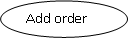
\includegraphics[width=1in]
{16}
\caption{Use Cases}
\end{figure}


\item {\bfseries Actors }

An actor represents a role that an outsider takes on when interacting with the business system. For instance, an actor can be a customer, a business partner, a supplier, or another business system and every actor has a name.
\item {\bfseries Dependency, generalization, and association relationships.}

A dependency is a semantic relationship between two things in which a change to one thing may affect the semantics of the other thing.

\begin{figure}[h!]
\centering
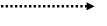
\includegraphics[width=1in]
{17}
\caption{Dependencies}
\end{figure}

A {\em generalization} is a relationship in which objects of specialized elements (the child) are substitutable for objects of the generalized element.
                 
An {\em association} is a structural relationship that describes a set of links, a link being connection among objects

Like all other diagrams, use case diagram may contain notes and constraints.
\end{itemize}


\begin{figure}[H]
\centering
\includegraphics[width=4in]
{usecase.pdf}
\caption{Use Case Diagram}
\end{figure}

\newpage

\subsection{Use-Case Scenario:}

\begin{center}
\begin{longtable}{|p{5cm}|p{9cm}|}
\hline
   {\bf USE CASES}     & {\bf USE CASE SCENARIO} \\ \hline
\endfirsthead   
\multicolumn{2}{c}%
{{\bfseries \tablename\ \thetable{} -- continued from previous page}} \\
    \hline
   {\bf USE CASES}     & {\bf USE CASE SCENARIO} \\ \hline
\hline
\endhead
\hline \multicolumn{2}{|r|}{{Continued on next page}} \\ \hline
\endfoot
\endlastfoot
\textbf{Register Student } & 1.  Open the student registration form.\\
& 2. Fill the own record of student like Roll No, Name, Year, Branch, Semester and  password. \\
& 3.  Click on register button.\\
& 4. Confirm the student registration.\\
& 5. Store into database.\\\hline
\textbf{Login} & 1.	Click on login button.\\
& 2.  Open login form.\\
& 3.  Login student with Roll number and Password.\\
& 4.  Student get login.\\\hline
\textbf{Register Face} & 1.  Open the OpenCV manager.\\
& 2.  Enter the face name.\\
& 3.  Capture the face and compare this face from database.\\
& 4.  If current captured face match with previous stored face into database then directly open the authentication form.\\\hline
\textbf{Mark Attendance} & 1. Click on Attendance Sheet form.\\
& 2. Fill the Subject name, Date and Roll no.\\
& 3. Click on Done button.\\
& 4.  Click on face recognition.\\  
& 5. Open the OpenCV manager and searching the face.\\
& 6.  If captured face is matched with previous stored face into database then mark attendance.\\
& 7.  Otherwise the student is absent.\\\hline
\textbf{Get Report} & 1. Click on Get report button.\\
& 2. Open Get report form.\\
& 3.  Enter the subject name.\\
& 4. Enter the date.\\
& 5.  Click on get report button\\
& 6.  It give the report of particular subject.\\\hline
%  \end{tabular}%
\caption{Use Case Scenario}
 \label{tab:addlabel}%
%\end{table}%
\end{longtable}
\end{center}
	
\section{Sequence Diagram: }
\subsection{Contents: }
{\bfseries Sequence diagram commonly contains: }
\begin{itemize}
\item Objects 
\item Links
\item Messages
\end {itemize}

\subsection{Description:}
A Sequence diagram is an interaction diagram that shows how processes operate with one another and in what order. It is a construct of a Message Sequence Chart. A sequence diagram shows object interactions arranged in time sequence. It depicts the objects and classes involved in the scenario and the sequence of messages exchanged between the objects needed to carry out the functionality of the scenario. Sequence diagrams are typically associated with use case realizations in the Logical View of the system under development. Sequence diagrams are sometimes called event diagrams or event scenarios.\cite{priti}
UML sequence diagrams are used to show how objects interact in a given situation. An important characteristic of a sequence diagram is that time passes from top to bottom: the interaction starts near the top of the diagram and ends at the bottom 

\begin{figure}[H]
\centering
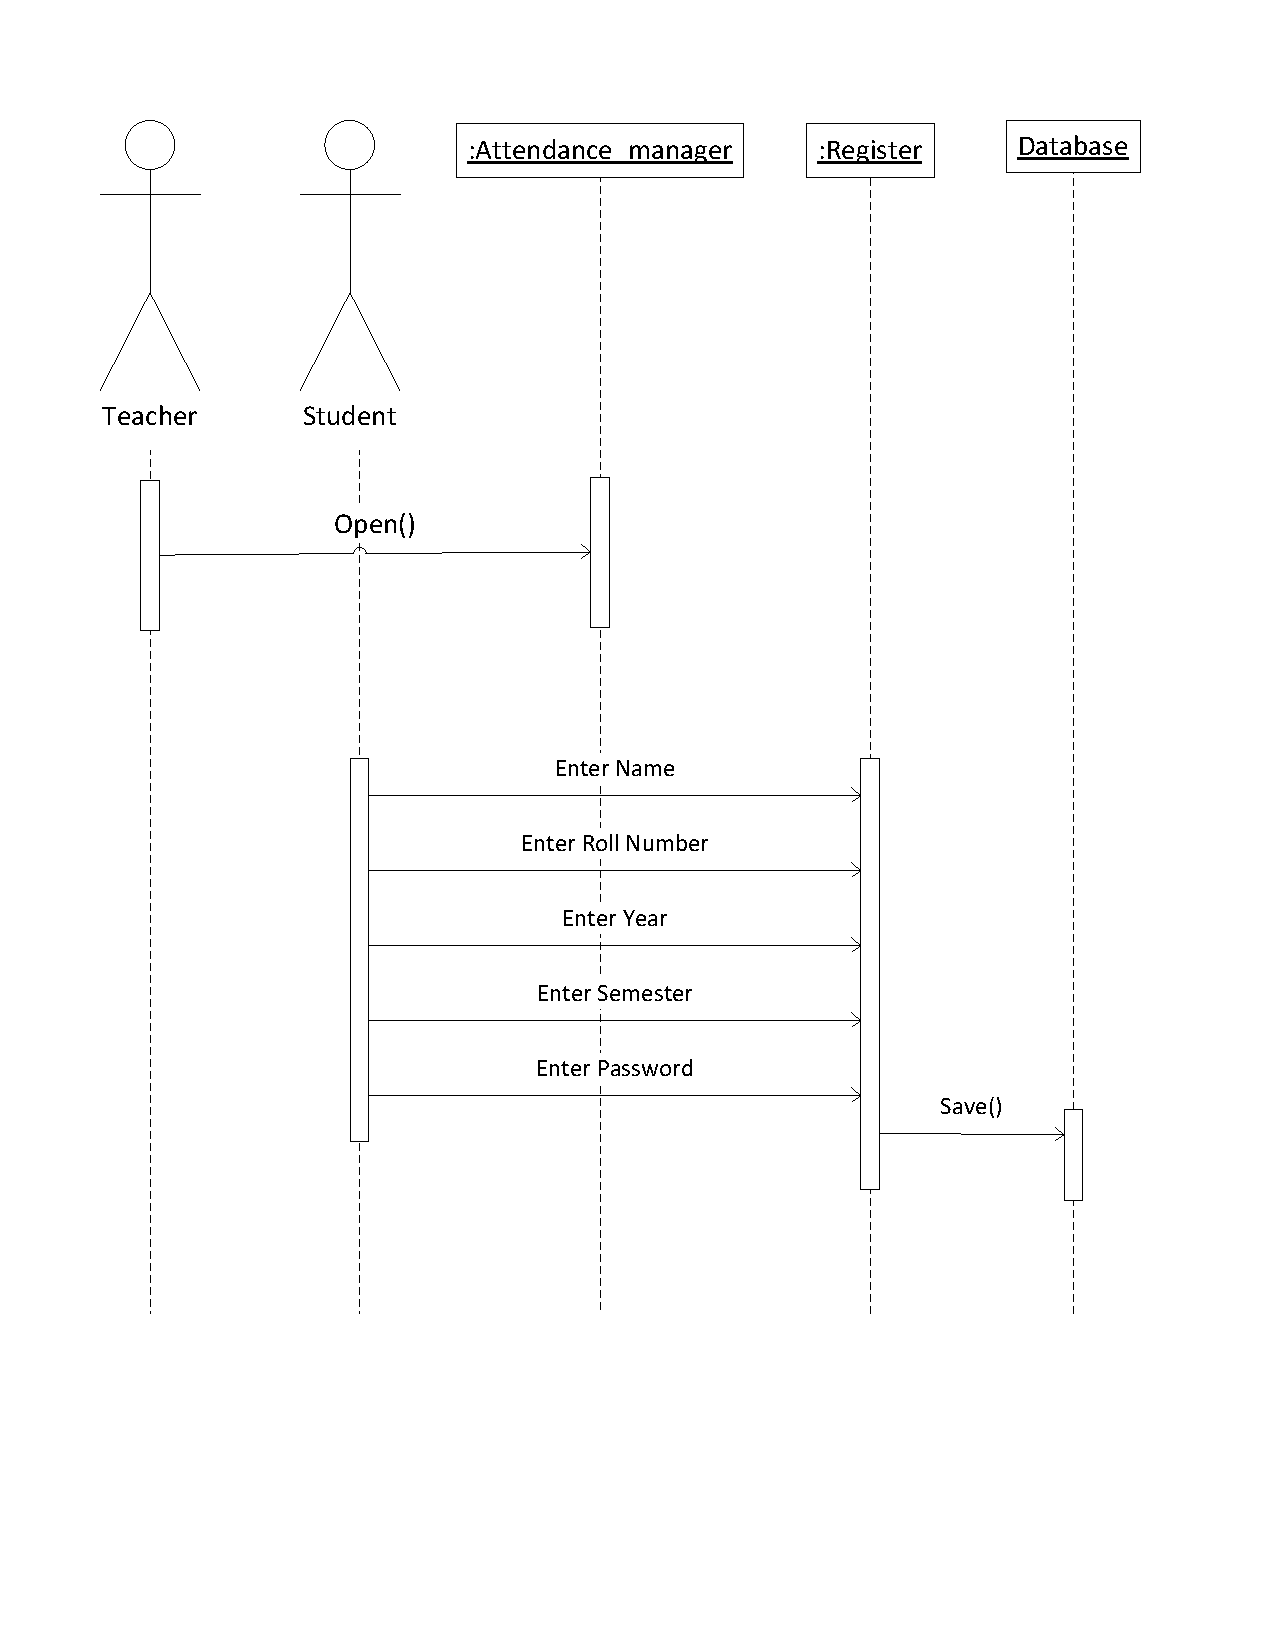
\includegraphics[width=6in]
{registration.pdf}
\caption{Student Registration Diagram}
\end{figure}

\begin{figure}[H]
\centering
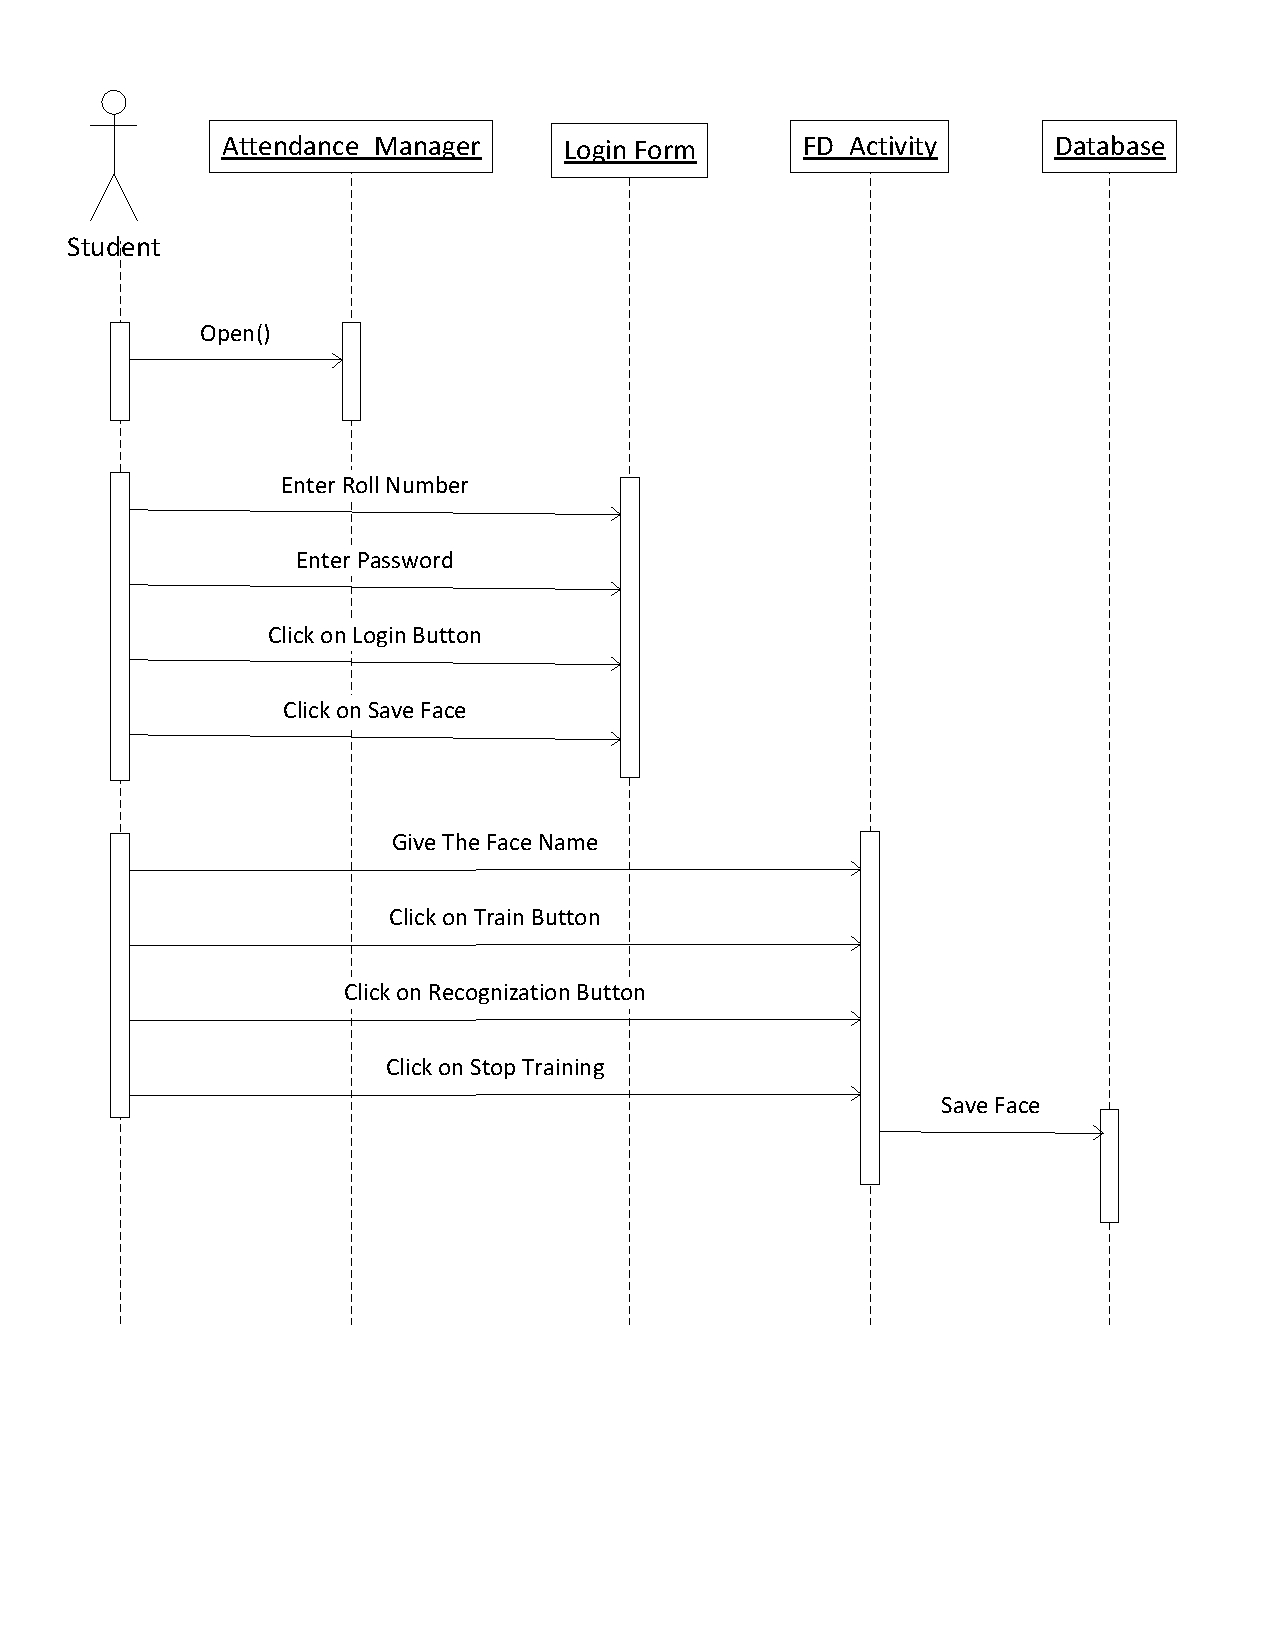
\includegraphics[width=6in]
{login.pdf}
\caption{Student Login}
\end{figure}

\begin{figure}[H]
\centering
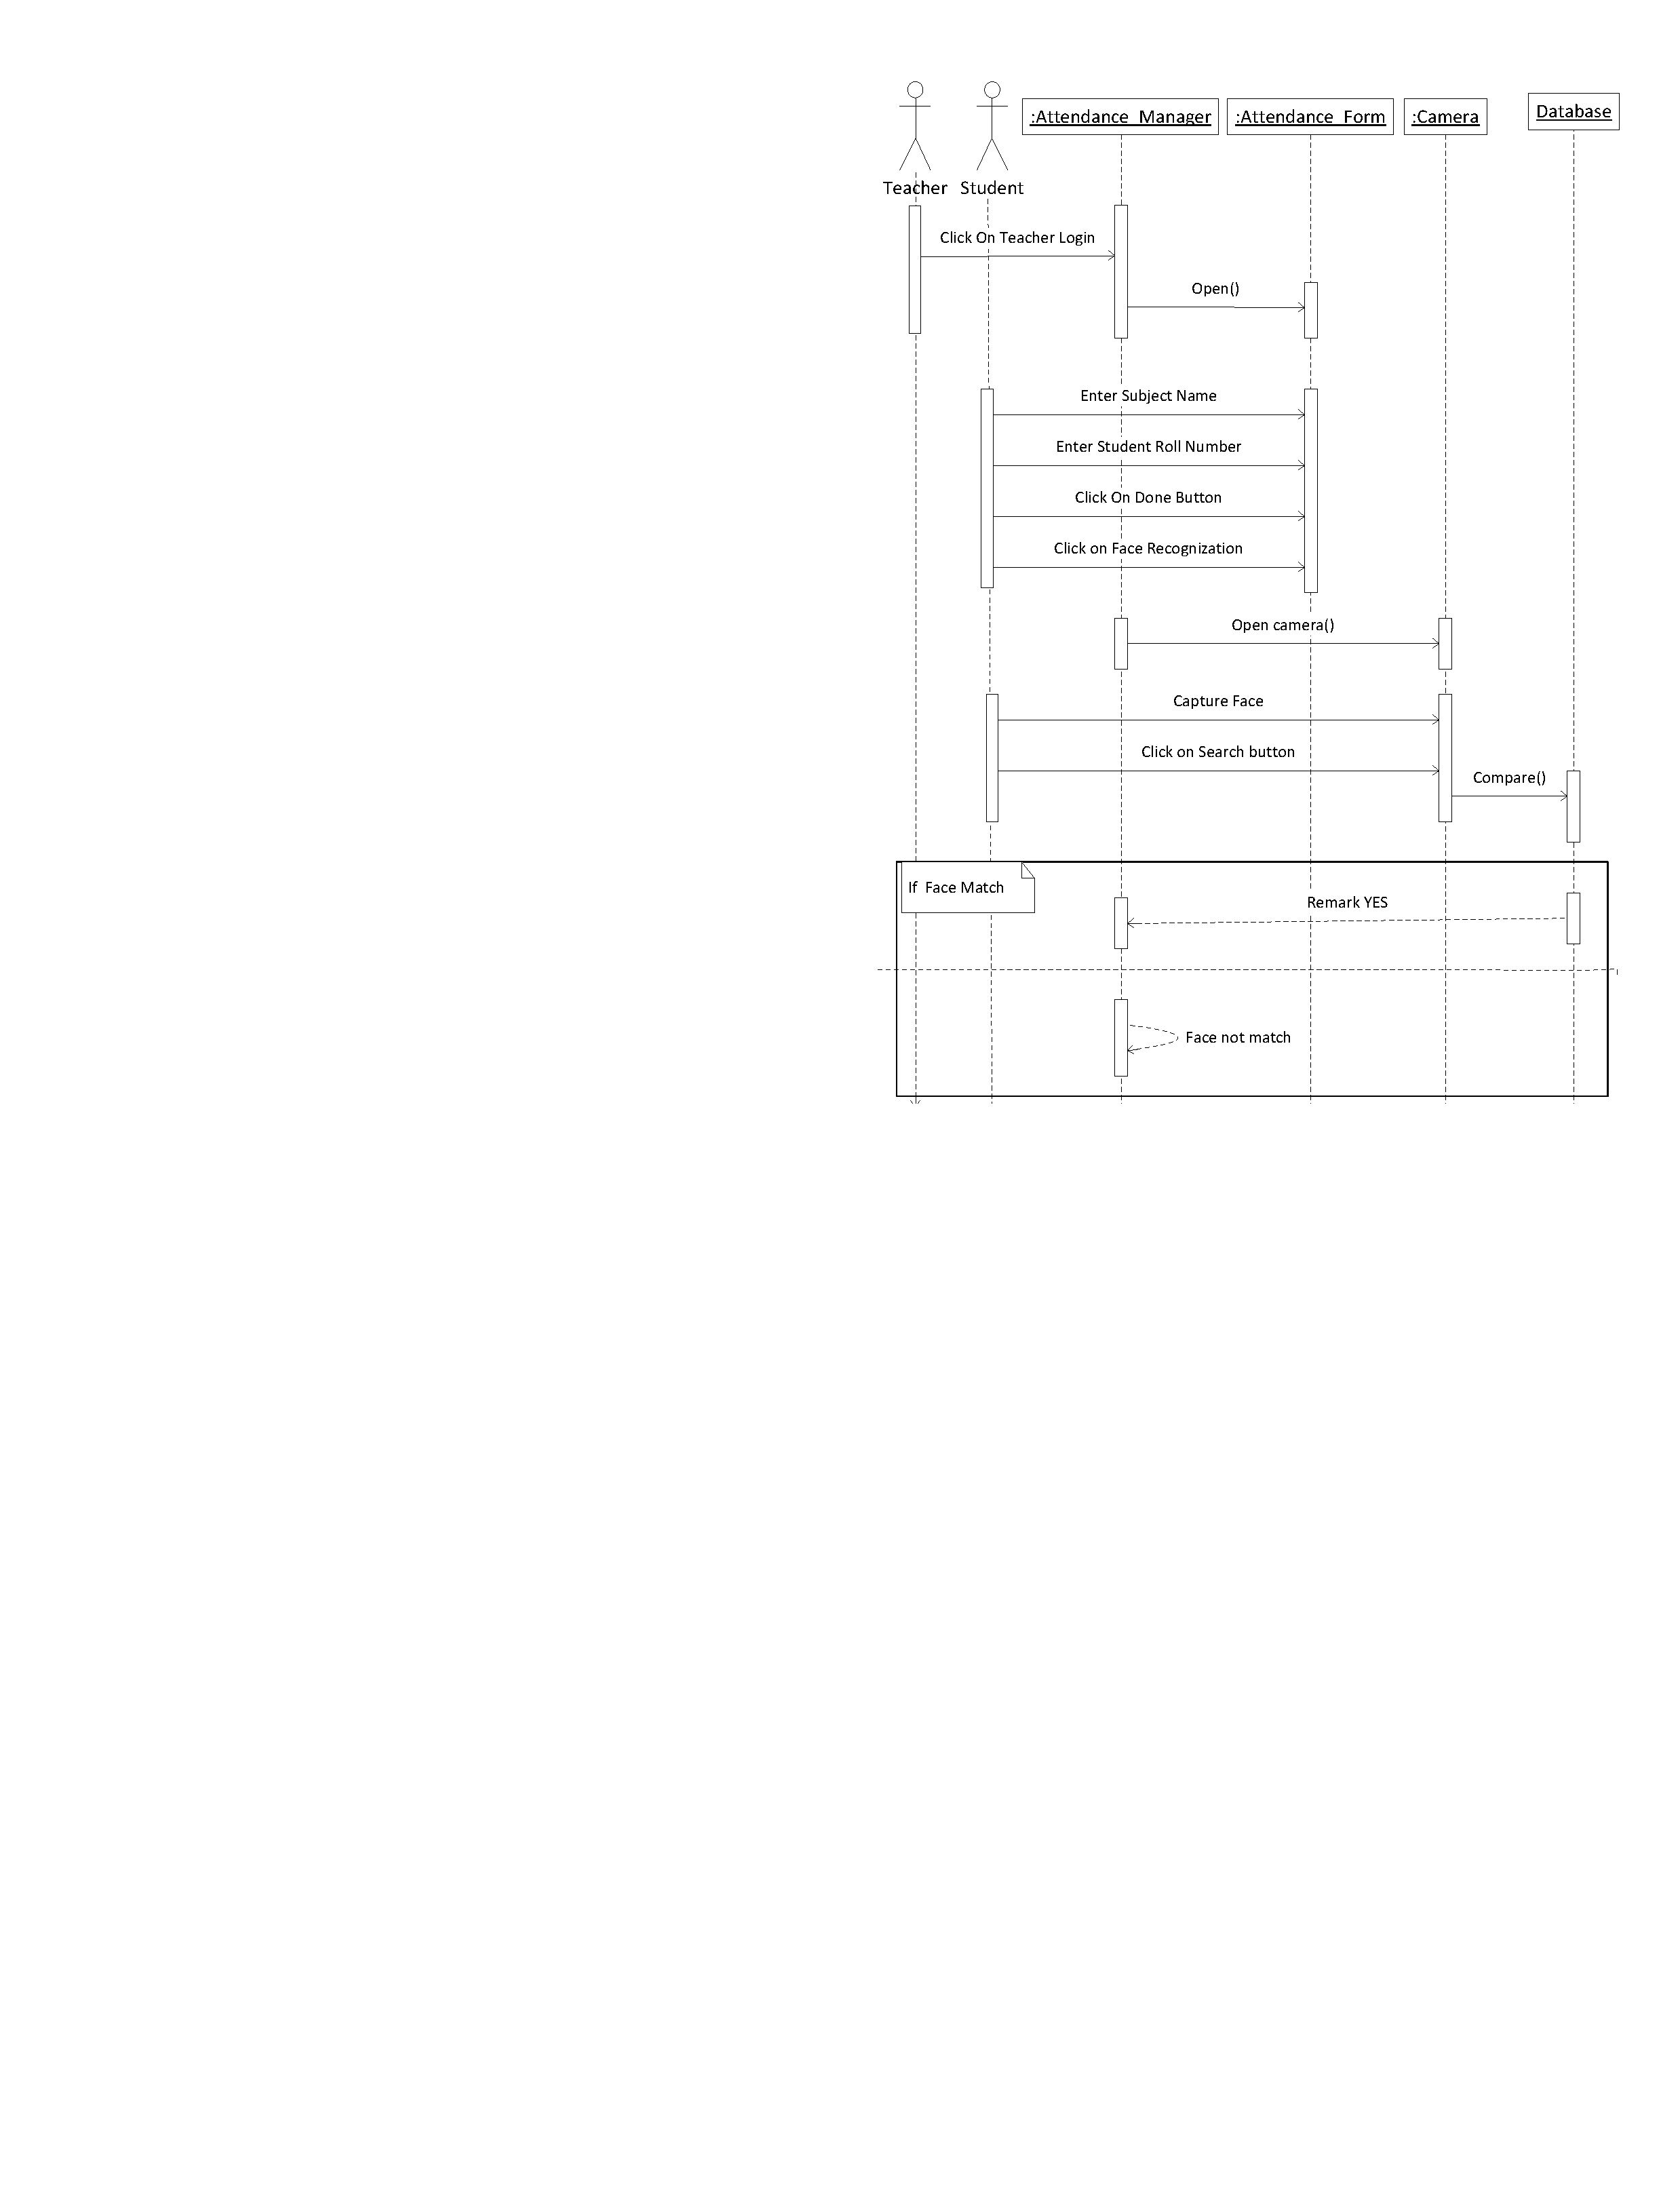
\includegraphics[width=6in]
{markatt.pdf}
\caption{Mark Attendance Sheet}
\end{figure}

\begin{figure}[H]
\centering
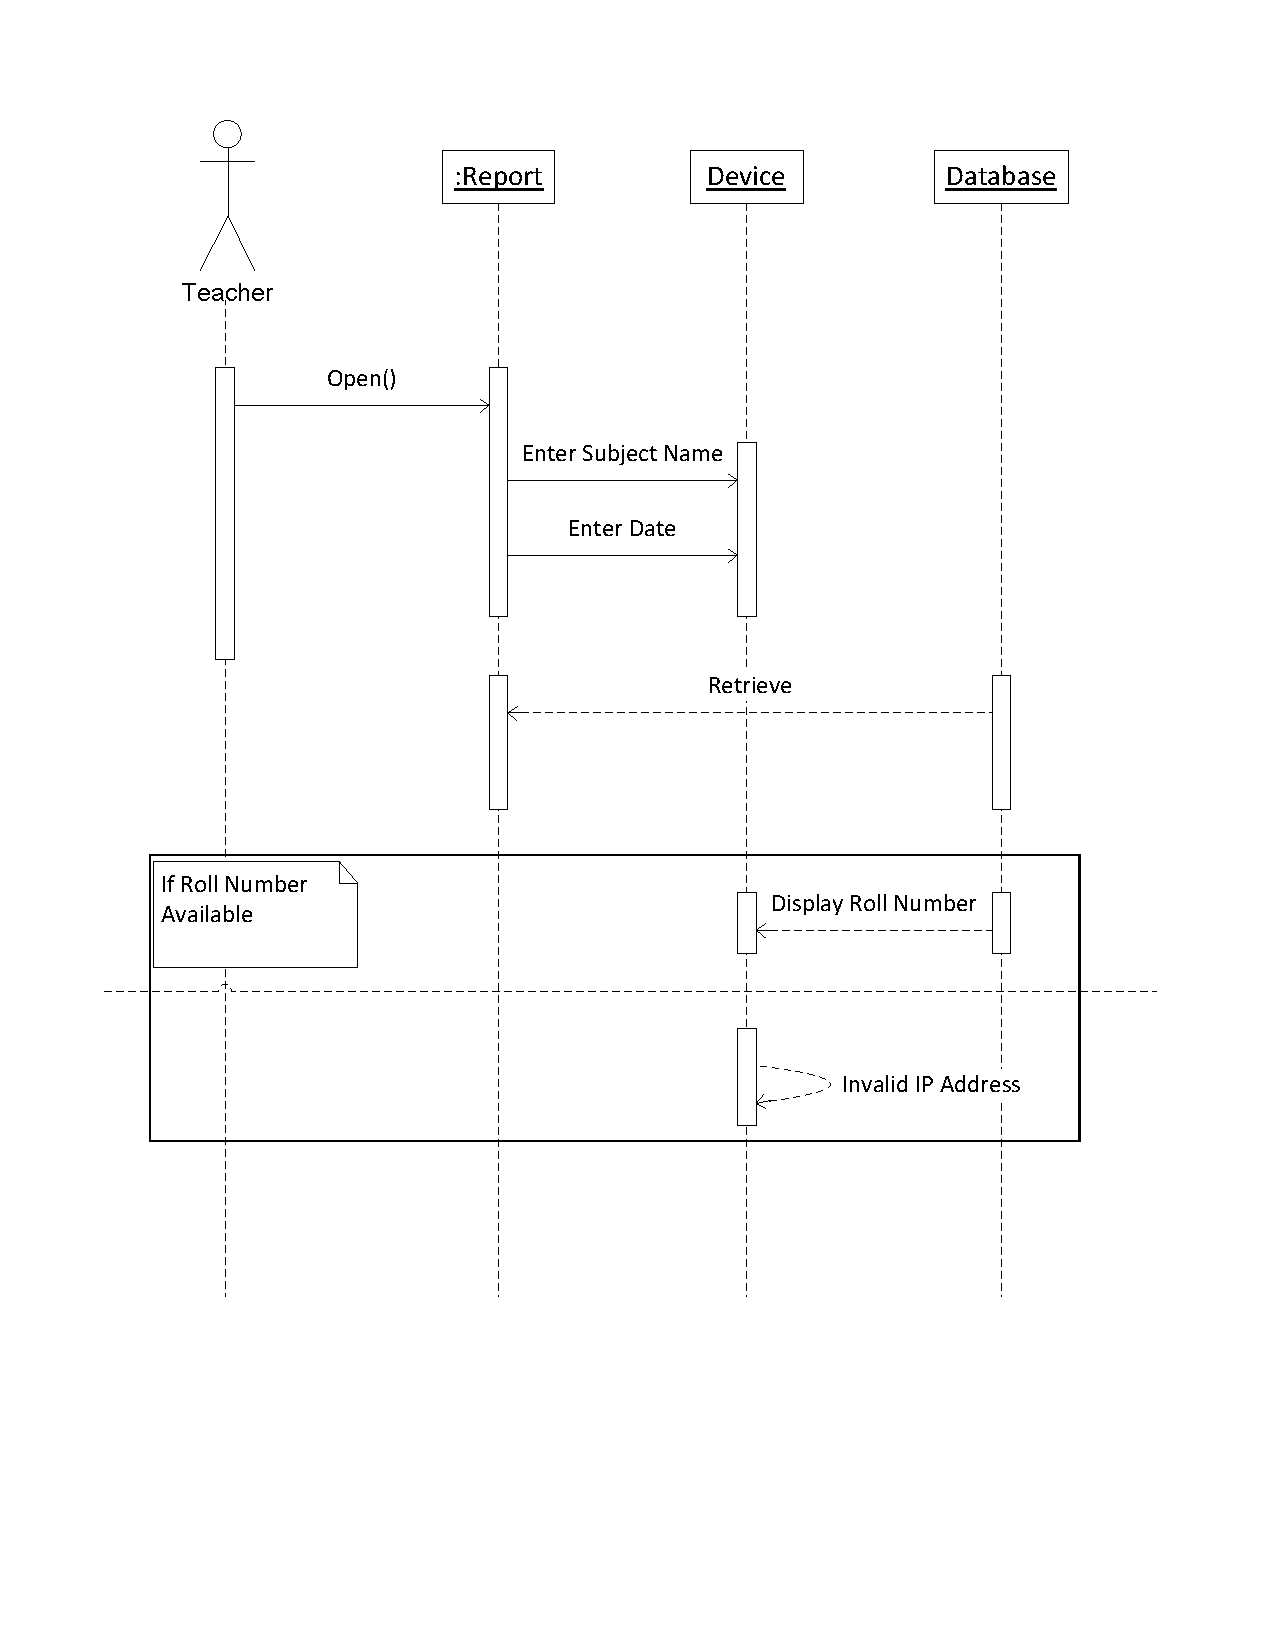
\includegraphics[width=6in]
{getreport.pdf}
\caption{Get Report}
\end{figure}

\newpage
\section{Class Diagram: }

\subsection{Contents: }
Class diagram commonly contain the following things:
\begin{itemize}
\item Classes 
\item Interfaces 
\item Collaborations
\item Dependency, generalization, and association relationships.
\end{itemize}

\subsection{Definition and Common Uses:}
A class diagram is a diagram that shows a set of classes, interfaces and their relationships. Graphically, a class diagram is a collection of vertices and arcs. A class diagram will shares the same common properties as do all other diagrams.
A class diagram is an illustration of the relationships and source code dependencies among classes in the Unified Modeling Language (UML). In this context, a class defines the methods and variables in an object, which is a specific entity in a program or the unit of code representing that entity. Class diagrams are useful in all forms of object-oriented programming (OOP). The concept is several years old but has been refined as OOP modeling paradigms have evolved.
In a class diagram, the classes are arranged in groups that share common characteristics. A class diagram resembles a flowchart in which classes are portrayed as boxes, each box having three rectangles inside. The top rectangle contains the name of the class; the middle rectangle contains the attributes of the class; the lower rectangle contains the methods, also called operations, of the class. Lines, which may have arrows at one or both ends, connect the boxes. These lines define the relationships, also called associations, between the classes.
\begin{itemize}
\item Class: A definition of objects that share given structural or behavioral characteristics.
\item Attribute: A typed value attached to each instance of a classifier.
\item Operation: A method or function that can be performed by instances of a classifier
\end{itemize}

\subsection{Description:}
A UML class diagram describes the object and information structures used by your application, both internally and in communication with its users. It describes the information without reference to any particular implementation. Its classes and relationships can be implemented in many ways, such as database tables, XML nodes, or compositions of software objects.[1]
\begin{itemize}
 \item                 Class: A definition of objects that share given structural or behavioral characteristics.
 \item               Attribute: A typed value attached to each instance of a classifier.
 \item                Operation: A method or function that can be performed by instances of a classifier.
\end{itemize}

\begin{figure}[H]
\centering
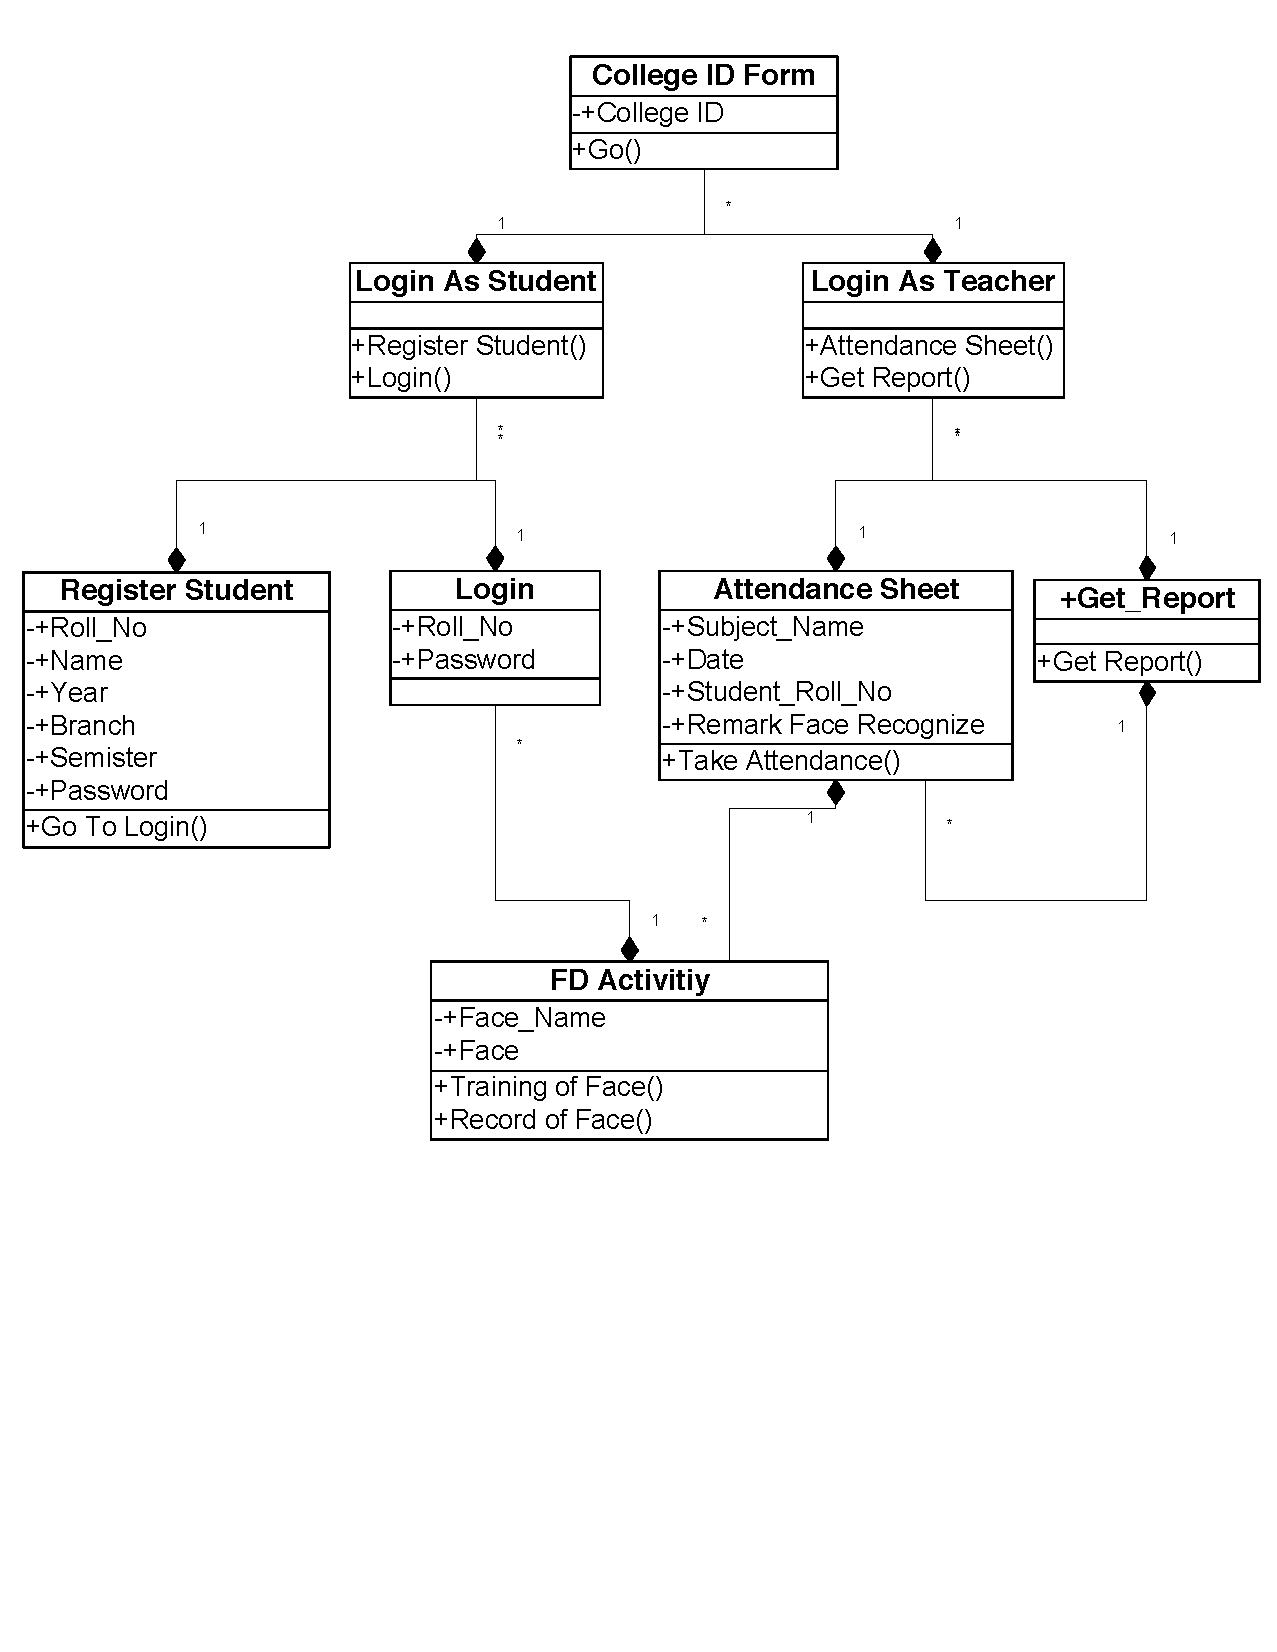
\includegraphics[width=6in]
{class.pdf}
\caption{Class Diagram}
\end{figure}

 \section{Deployment Diagram: }
\subsection{Definition: }
A deployment diagram shows the configuration of run time processing nodes and the components that live on them. Deployment diagram address the static deployment view of architecture. They are related to component diagrams in that a node typically encloses one or more componentsThe name Deployment itself describes the purpose of the diagram. Deployment diagrams are used for describing the hardware components where software components are deployed. Component diagrams and deployment diagrams are closely related.
The purpose of deployment diagrams can be described as:
\begin{itemize}
\item             Visualize hardware topology of a system.
\item               Describe the hardware components used to deploy software components.
\item              Describe runtime processing nodes.
\end{itemize}	
Deployment diagrams are useful for system engineers. An efficient deployment diagram is very important because it controls the following parameters:

\begin{itemize}
\item               Performance
\item              Scalability
\item                Maintainability
\item Portability
\end{itemize}
So before drawing a deployment diagram the following artifacts should be identified:

\begin{itemize}
\item                 Nodes
\item             Relationships among nodes
\end{itemize}

\newpage
The following deployment diagram is a sample to give an idea of the deployment view of order management system. Here we have shown nodes as:
\begin{itemize}
\item                 Monitor
\item            Modem
\item              Caching server
\item Server
\end{itemize}

\begin{figure}[H]
\centering
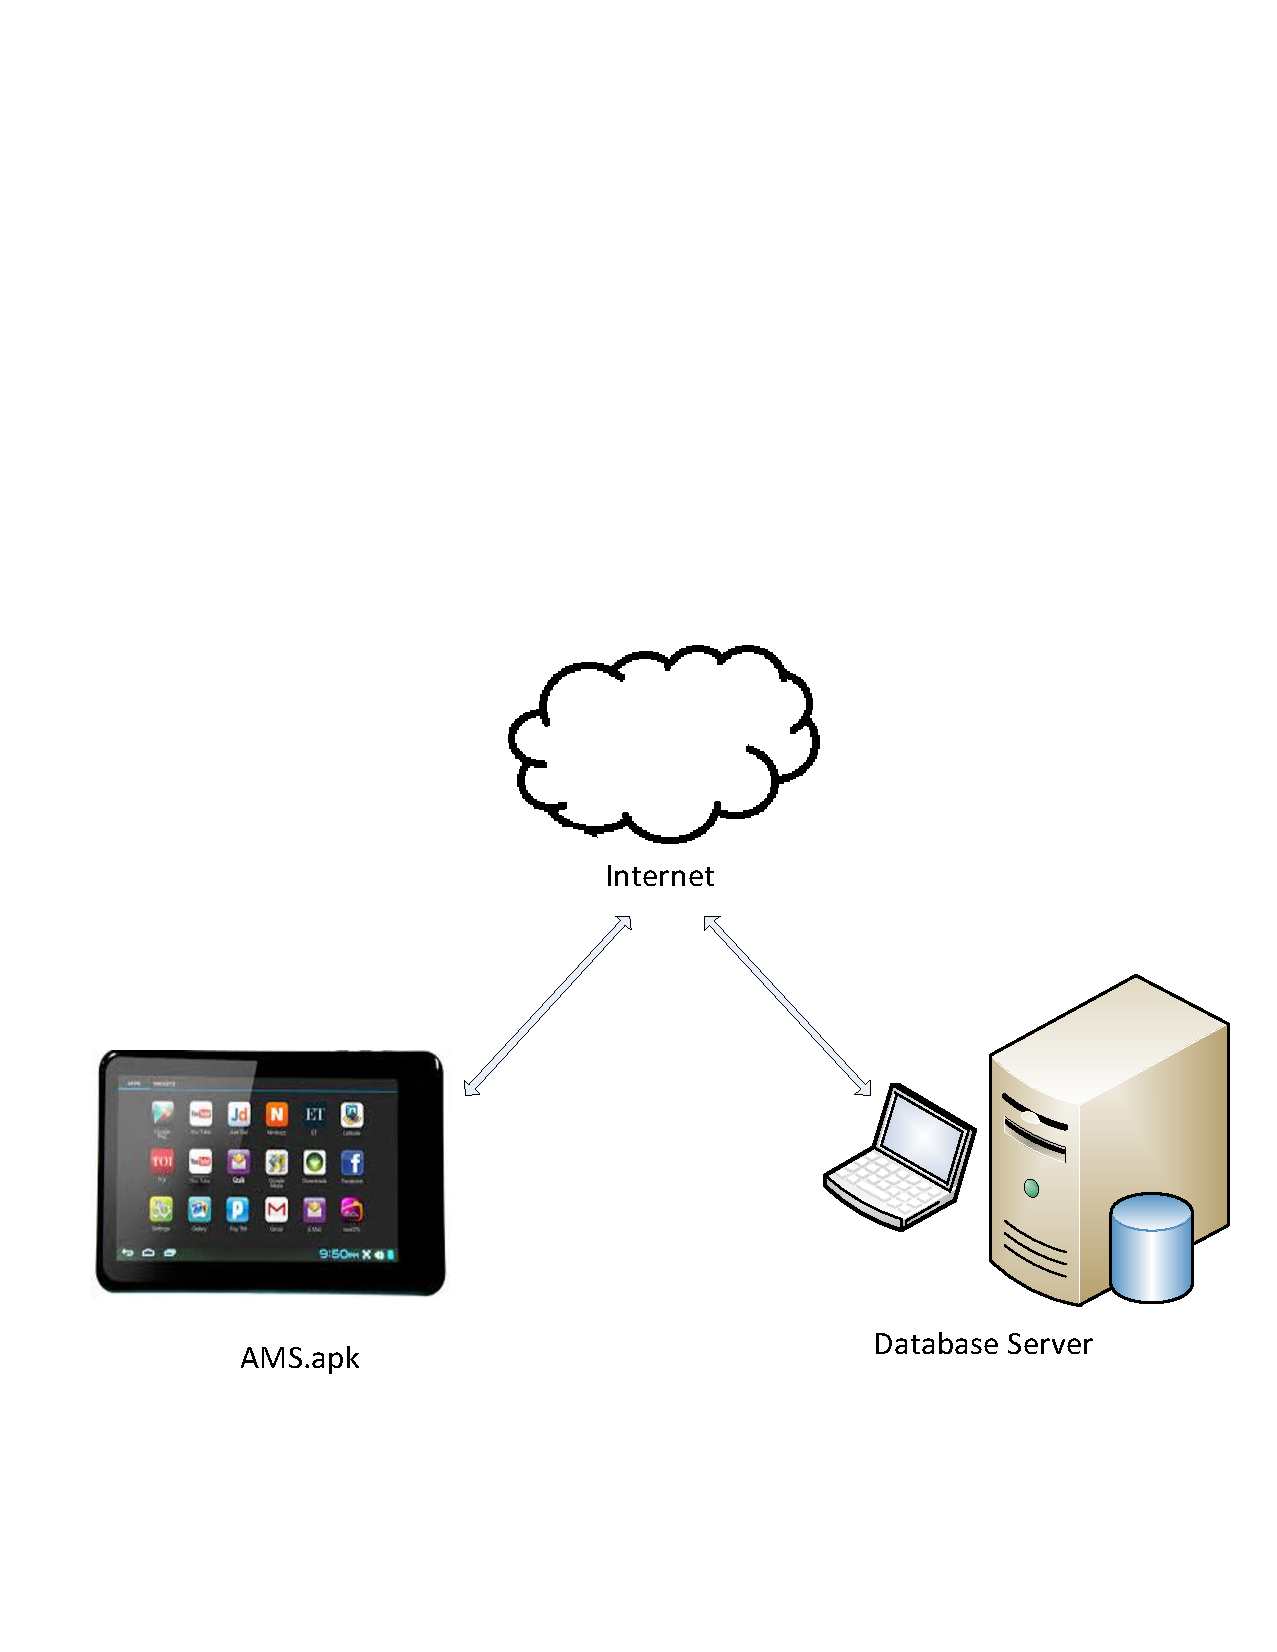
\includegraphics[width=4in]
{deploy.pdf}
\caption{Deployment Diagram}
\end{figure}








